\subsubsection{14.01.15}
\begin{enumerate}
	
	\item Time of beginning and ending of meeting: 18:10 - 21:00.
	
	\item Purposes of meeting: 
	\begin{enumerate}
		
		\item To move the crossbar that fixed stationary higher.
		
	\end{enumerate}

	\item Work that has been done:
	\begin{enumerate}
		
		\item In Ryazan it was found that the lift shakes during the rising. It was found out that it happens due to that the bottom crossbar that fixed on the bottom slat rises higher than the stationary crossbar. So the bottom slat rises not fully but it tries to rise during the extracting the lift. So the lift shakes. To prevent this it was decided to move the stationary crossbar higher. So that the bottom slat raises fully and lift doesn't shakes.
        \begin{figure}[H]
	  	  \begin{minipage}[h]{0.2\linewidth}
	  	    \center  
	  	  \end{minipage}
	  	  \begin{minipage}[h]{0.6\linewidth}
	  		\center{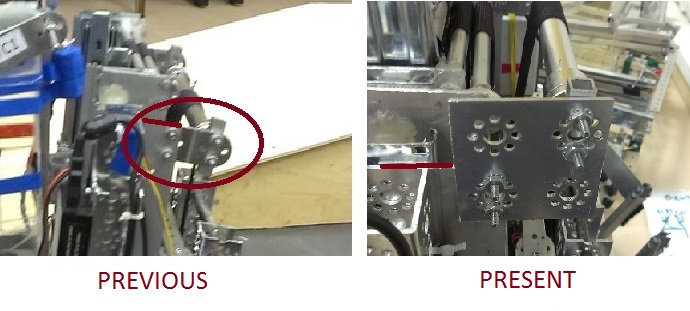
\includegraphics[scale=0.35]{days/14.01.15/images/01}}
	  		\caption{The new mount of crossbar}
	  	  \end{minipage}
	   \end{figure}

	\end{enumerate}
	
	\item Results:
	\begin{enumerate}
		
		\item Crossbar was moved higher but lift wasn't tested.
		
	\end{enumerate}
	
	\item Tasks for the next meetings:
	\begin{enumerate}
		
		\item To train on the control robot.
		
		\item To test the lift.
			
	\end{enumerate}
\end{enumerate}
\fillpage
